\chapter{L'azienda}
\label{cap:lazienda}


\section\azienda

\subsection{Descrizione dell'azienda}
Nata nel 1984, \azienda{} rappresenta oggi una realtà di primo piano nel panorama della consulenza e dello sviluppo \textit{software}. 
Vanta un portfolio con oltre 2500 clienti, tra cui spiccano nomi di rilievo internazionale. \\
L'impegno verso la clientela è il pilastro su cui si fonda l'azienda, che si estende con uffici in molteplici 
regioni italiane: dal Veneto alla Lombardia, passando per Emilia-Romagna, Friuli-Venezia Giulia, Toscana, Puglia e 
Campania. Un \textit{team} di oltre 600 professionisti, altamente qualificati, costituisce la forza lavoro di \azienda. \\
Il fulcro dell'innovazione è localizzato nel Centro di Sviluppo e Ricerca (CSV) a Grisignano di Zocco (VI). 
Qui, più di 200 tra sviluppatori e tecnici lavorano in sinergia per creare soluzioni \textit{software} su misura, 
efficienti e affidabili, progettate per soddisfare le esigenze specifiche di ogni cliente. \\


\subsection{Organizzazione e prodotti}
L'organizzazione di \azienda{} è strutturata in diverse \textit{Business Unit} (BU), ciascuna con una visione, \textit{mission}, strategie e obiettivi specifici. Operando in modo autonomo o semi-autonomo, 
queste unità hanno una struttura organizzativa propria e sono responsabili dei loro bilanci economici, permettendo una focalizzazione mirata su mercati geografici, gruppi di clienti specifici. 
Questa struttura rende \azienda{} agile e reattiva alle dinamiche di mercato. \\
Le BU in \azienda{} sono 11, distinte per aree di specializzazione, come illustrato in figura \ref{fig:organizzazione-azienda}:
\begin{itemize}
\item \textbf{JGALILEO:} offre l’\textit{\gls{ERP}} Jgalileo, un sistema di gestione integrato che ottimizza i processi aziendali per imprese di varie dimensioni, con un focus sulle normative fiscali internazionali;
\item \textbf{NEXTBI:} si concentra su \textit{Information Technology} e consulenza strategica, specializzandosi in \textit{marketing}, vendite, \textit{retail}, innovazione cliente, \textit{Business Intelligence} e soluzioni \gls{IoT};
\item \textbf{4WORDS:} fornisce soluzioni \textit{\gls{B2B}}, app e \textit{\gls{CRM}}, per potenziare il \textit{business} attraverso strumenti digitali, inclusi portali B2B e realtà aumentata;
\item \textbf{TCE:} si dedica alla semplificazione delle fasi di preventivazione e acquisizione ordini con il prodotto \gls{CPQg}, che permette di configurare prodotti e servizi in modo rapido e preciso;
\item \textbf{DISCOVERY QUALITY:} sviluppa \textit{software} per la \textit{Governance} aziendale, controllo dei processi e misurazione delle performance, con un occhio alle normative e metriche di sostenibilità (\gls{SDGs}, \gls{BCorp}), per garantire la qualità dei prodotti e servizi;
\item \textbf{ECM:} propone soluzioni di \gls{ECM} per la gestione efficace dei documenti digitali, fornendo strumenti per la gestione dei contenuti, la collaborazione e la condivisione dei documenti;
\item \textbf{SMITECH:} focalizzata sulla \textit{\gls{cybersecurity}} e protezione dei dati, offrendo servizi di consulenza, formazione e soluzioni tecnologiche per la sicurezza informatica;
\item \textbf{ELEMENT:} è la divisione creativa per lo sviluppo di siti \textit{web} ed \textit{e-commerce}, con un focus sull'esperienza utente e l'interfaccia grafica;
\item \textbf{JPA:} sviluppa \textit{software} di \gls{BPM} per l'automazione e integrazione dei processi aziendali, sviluppa una piattaforma per la gestione dei processi aziendali, fornendo un \textit{designer}  grafico per la modellazione dei processi, un motore di esecuzione per l'esecuzione dei processi ed un'interfaccia grafica per l'esecuzione dei \textit{task} assegnati agli utenti;
\item \textbf{FACTORY:} risponde alle esigenze della \gls{Supply Chain} con soluzioni per la fabbrica del futuro, mirate a ottimizzare il servizio clienti, \textit{asset} e profitti. Offre anche soluzioni per la gestione dei magazzini e per la gestione della produzione; 
\item \textbf{JPM:} offre soluzioni di \textit{\gls{Project Management}} per la gestione dei progetti, fornendo strumenti per la pianificazione, il monitoraggio e il controllo dei progetti che lavorano a commessa o a preventivo.
\end{itemize}

\begin{figure}[!h] 
  \centering 
  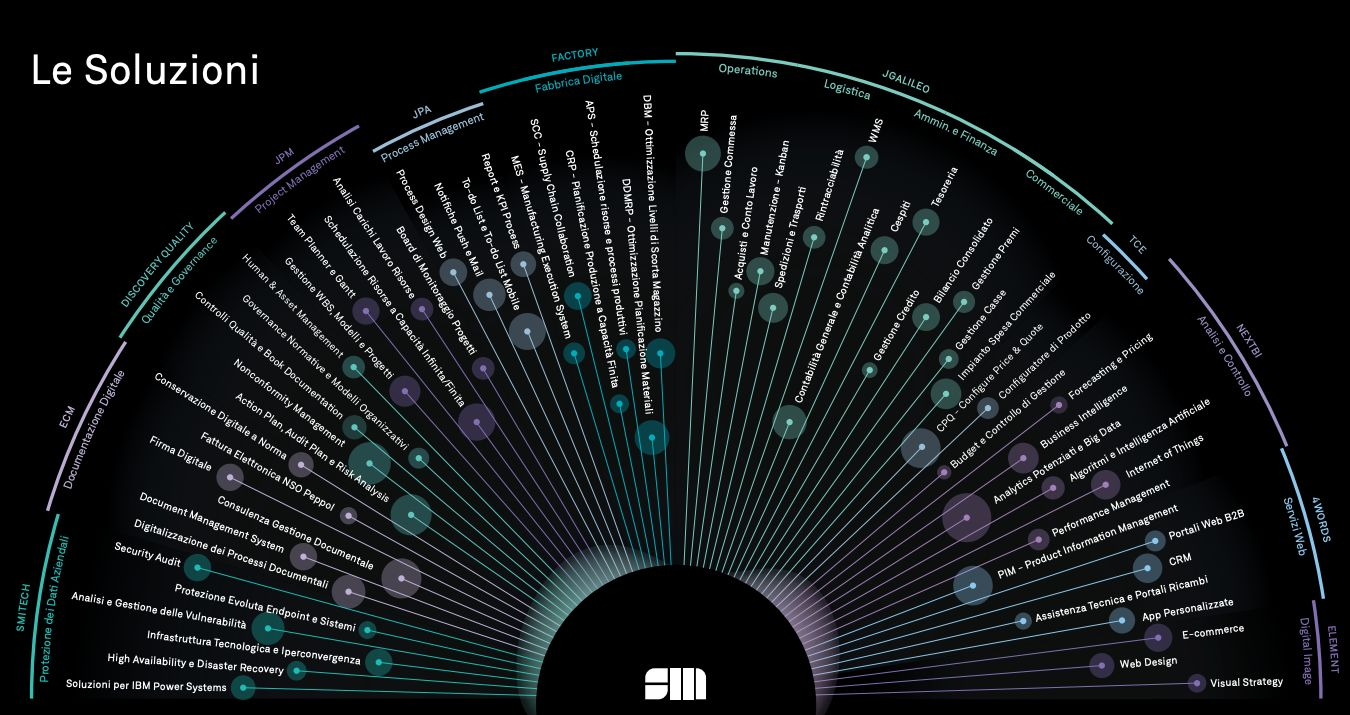
\includegraphics[width=1\columnwidth]{organizzazione-azienda} 
  \caption{Le BU di {\azienda} ed i loro Prodotti. Fonte: \url{https://www.sanmarcoinformatica.it/intranet.pag}}
  \label{fig:organizzazione-azienda}
\end{figure}


\subsection{Strategie e obiettivi}
Il piano strategico triennale di \azienda{}, battezzato \textit{Vision 2025}, è un manifesto per la crescita sostenibile, l'innovazione continua e la piena 
soddisfazione del cliente. Il piano si colloca tra ambizione commerciale e responsabilità sociale, mirando a rafforzare la posizione 
di \azienda{} come \textit{leader}  nel settore informatico, sia a livello nazionale che internazionale. \\ 
L'obiettivo principale di \textit{Vision 2025} è di espandere la penetrazione di mercato di \azienda{}, non solo consolidando la sua presenza nei mercati italiani, 
ma anche esplorando nuove opportunità in ambito internazionale. Un'attenzione particolare è rivolta ai mercati emergenti e in rapida espansione, come quelli 
nordamericani e asiatici, dove la domanda di soluzioni informatiche innovative è in costante crescita. \\ 
Per realizzare questa visione, \azienda{} si impegna in un investimento strategico nelle tecnologie più avanzate,
includendo l'adozione di nuove piattaforme \textit{software}, l'aggiornamento delle infrastrutture esistenti e l'esplorazione 
di nuove frontiere nell'ambito dell'intelligenza artificiale e del big data. Inoltre, un'enfasi particolare è posta sul potenziamento delle competenze dei 
\textit{team} di \azienda{}, attraverso programmi di formazione continua e l'assunzione di talenti nel campo dell'informatica, garantendo che l'azienda rimanga 
all'avanguardia nell'innovazione tecnologica. \\ 
Parallelamente, \azienda{} si impegna a promuovere la responsabilità sociale d'impresa. 
Questo si traduce nel rispetto dei \gls{SDGs} e nella ricerca della certificazione \gls{BCorp}, che riconosce le aziende per il loro impatto positivo 
sia sociale che ambientale. L'impegno riflette la consapevolezza di \azienda{} sull'importanza di operare in modo etico e sostenibile, riconoscendo
 che il successo aziendale che va di pari passo con il benessere della comunità e dell'ambiente. \\ 
 Infine, \azienda{} prevede di ampliare il proprio portafoglio prodotti, introducendo soluzioni \textit{software} innovative che rispondano alle esigenze in continua evoluzione del mercato. 
 Questo include lo sviluppo di nuove applicazioni, l'aggiornamento e il miglioramento delle soluzioni esistenti e l'espansione in nuovi segmenti di mercato. 
 L'obiettivo è di garantire che ogni cliente riceva soluzioni personalizzate che offrano il massimo valore aggiunto, 
 consolidando così la posizione di \azienda{} come \textit{leader}  nel settore delle soluzioni informatiche.

 \subsubsection{\textbf{La \textit{Business unit}}}

 \noindent Nell'ecosistema di \azienda{}, le \textit{Business Unit} (BU) rappresentano, non solo divisioni funzionali, ma veri e propri centri di innovazione e sviluppo agile. 
 Ogni BU, con la sua struttura unica, è progettata per rispondere dinamicamente ai cambiamenti del mercato informatico, enfatizzando la collaborazione e la flessibilità. 
 L'approccio agile si traduce in una consegna incrementale di valore, dove il \textit{feedback} continuo e l'adattamento alle esigenze emergenti sono fondamentali.
 
 \noindent La gestione dei progetti all'interno delle BU è un esercizio di equilibrio tra innovazione e efficienza. I responsabili di progetto giocano un ruolo cruciale, 
 bilanciando il \textit{budget}, le risorse umane e le aspettative dei clienti. 
 La gestione richiede una comprensione profonda delle tecnologie emergenti e delle metodologie di sviluppo \textit{software}, 
 assicurando che ogni progetto, non solo rispetti i tempi e i costi, ma sia anche all'avanguardia in termini di soluzioni tecnologiche.
 
 \noindent All'interno di ogni BU, il \gls{PO} è la figura chiave che assicura l'allineamento del progetto con le visioni e gli obiettivi del cliente. 
 Lavorando a stretto contatto con gli sviluppatori, il PO traduce le esigenze del cliente in requisiti tecnici, garantendo che il prodotto finale soddisfi o superi le aspettative. 
 Lo \gls{Scrum Master}, d'altra parte, si concentra sull'ottimizzazione dei processi di sviluppo, assicurando che il \textit{team} adotti le migliori pratiche agili e mantenga un alto 
 livello di produttività.
 
 \noindent Gli sviluppatori, con le loro competenze tecniche, sono il motore che alimenta l'innovazione all'interno di \azienda. 
 Lavorando su una vasta gamma di tecnologie, da Java e Angular a soluzioni \textit{cloud} e \textit{mobile}, sono in prima linea nel trasformare le idee in realtà tangibili. 
 I \textit{tester}, collaborando strettamente con gli sviluppatori, assicurano che ogni prodotto sia robusto e privo di errori, un aspetto cruciale in un settore dove 
 la qualità del \textit{software} è direttamente correlata alla soddisfazione del cliente.
 
 \noindent I consulenti e gli \gls{analisti} svolgono un ruolo fondamentale nell'interpretare le esigenze del cliente e nel tradurle in specifiche tecniche. 
 Il lavoro di analisi è vitale per garantire che i progetti siano allineati con le aspettative del cliente e con le tendenze del mercato.
 
 \noindent Oltre alle BU, la struttura organizzativa di \azienda{} comprende vari dipartimenti che supportano le operazioni quotidiane. 
 Il dipartimento delle risorse umane si occupa di attrarre e mantenere talenti, essenziale in un settore in rapida evoluzione come l'informatica. 
 Il \textit{marketing}, attraverso strategie digitali e tradizionali, posiziona \azienda{} sul mercato, mentre l'Amministrazione garantisce la solidità finanziaria. 
 Il dipartimento \gls{IT}, con il suo ruolo di supporto e innovazione, è il cuore tecnologico dell'azienda, garantendo che l'infrastruttura informatica sia sempre efficiente e all'avanguardia.
 
 \noindent In conclusione, la struttura di \azienda{} è un tessuto complesso di competenze e funzioni, tutte orientate verso l'obiettivo comune di eccellenza nel settore informatico. 
 Questa sinergia tra le diverse unità e dipartimenti è ciò che permette a \azienda{} di rimanere competitiva e innovativa in un mercato in costante evoluzione.
 
\subsubsection*{Monitoraggio delle attività}
\noindent La struttura lavorativa in \azienda{} è caratterizzata da una flessibilità che si adatta alle esigenze moderne del settore informatico. 
Con un \textit{team} distribuito che include dipendenti in sede, personale in lavoro remoto e professionisti che operano direttamente presso i clienti, 
\azienda{} adotta un approccio moderno e versatile alla gestione del lavoro. 
La diversità nelle modalità lavorative riflette la dinamicità del settore IT e la necessità di un approccio agile e personalizzato per 
ogni progetto.

\noindent Per coordinare efficacemente la forza lavoro distribuita, \azienda{} si affida a un sofisticato \textit{software} interno di 
\textit{time tracking}. Questo strumento è fondamentale per garantire trasparenza e precisione nella registrazione delle ore lavorative. 
Ogni dipendente, dotato di un proprio \textit{account} personale, registra le ore dedicate a specifici progetti, 
fornendo così una visione chiara del tempo impiegato in ogni attività. Il sistema, non solo facilita la gestione amministrativa, 
ma è anche uno strumento prezioso per la pianificazione e l'allocazione delle risorse.

\noindent Il processo di inserimento delle ore lavorate è dettagliato e strutturato per catturare tutte le informazioni rilevanti. 
Durante la compilazione del "rapportino", il dipendente inserisce una descrizione dettagliata delle attività svolte, specificando la commessa, 
l'eventuale cliente, la sede di lavoro e gli orari di inizio e fine attività. La procedura, che deve essere completata quotidianamente, 
permette di collegare ogni ora lavorata a specifici \textit{ticket} o progetti, assicurando una tracciabilità completa e una gestione efficiente del lavoro.

\noindent Al termine di ogni mese, il sistema blocca le ore registrate, consentendo ai responsabili di progetto e al dipartimento amministrativo 
di analizzare i dati raccolti. Questi report mensili sono essenziali per valutare la produttività, pianificare le risorse future e ottimizzare 
i processi lavorativi. Inoltre, il sistema di \textit{time tracking} gioca un ruolo cruciale nella trasparenza verso i clienti, 
fornendo una base solida per la fatturazione e la rendicontazione delle attività svolte.

\noindent In sintesi, la gestione del lavoro in \azienda{} è un esempio di come le tecnologie moderne possano essere impiegate per 
ottimizzare la gestione delle risorse umane in un contesto lavorativo complesso e diversificato. Questo approccio, non solo migliora 
l'efficienza operativa, ma contribuisce anche a una maggiore soddisfazione dei dipendenti e dei clienti, elementi fondamentali per il 
successo nel settore informatico.


\section{Il \textit{team} di sviluppo}

Durante il mio periodo in \textit{JPA} (\textit{Process Management}), ho avuto l'opportunità di osservare da vicino il lavoro di un \textit{team} di sviluppo particolarmente versatile. 
Il \textit{team}, a differenza di quelli più tradizionali focalizzati su un singolo prodotto, aveva l'obiettivo di fornire supporto globale a tutti i \textit{team} di sviluppo dell'azienda.
\noindent Il supporto tecnico e analitico era la principale attività del \textit{team}, affrontando e risolvendo problemi complessi per agevolare il lavoro degli altri \textit{team}. 
Questo ruolo cruciale implicava l'identificazione e la soluzione di sfide tecniche, assicurando un ambiente di sviluppo efficiente e senza ostacoli. \\
\noindent Un altro aspetto centrale del lavoro del \textit{team} era la formazione. Con l'evolversi continuo delle tecnologie e degli strumenti, era essenziale mantenere i \textit{team} aggiornati. Di conseguenza, il \textit{team} organizzava regolarmente sessioni di formazione per condividere conoscenze e competenze su nuove tecnologie e metodologie di sviluppo. \\
\noindent In parallelo, il \textit{team} era impegnato in attività di ricerca e sviluppo, in particolare nello sviluppo di un \textit{\gls{frameworkg}} interno. Il framework, un insieme di librerie e strumenti per lo sviluppo di applicazioni \textit{web}, era progettato per rendere la creazione di applicazioni \textit{web} più semplice e veloce, contribuendo significativamente all'efficienza dello sviluppo \textit{software} in azienda. \\
\noindent L'automazione dei processi di sviluppo era un'altra area chiave, includeva l'automazione della compilazione, il rilascio dei prodotti e lo sviluppo di nuove funzionalità, riducendo il tempo e lo sforzo necessari per le operazioni di \textit{routine}. \\
\noindent La gestione dei \textit{\gls{repository}} di codice sorgente e il supporto all'uso di strumenti di \textit{\gls{continuous_integrationg}} erano compiti fondamentali del \textit{team}; assicurava una gestione efficace del codice e un'integrazione continua, elementi vitali per mantenere la qualità e l'affidabilità del \textit{software}. \\
\noindent Infine, il \textit{team} era responsabile dello sviluppo di un installatore per i prodotti dell'azienda basati sul \textit{\gls{frameworkg}} interno. Lo strumento semplificava il processo di installazione, rendendo i prodotti più accessibili agli utenti finali. \\
\noindent Il \textit{team} era composto da tre persone: uno \gls{Scrum Master} e due sviluppatori. In questo ambiente dinamico, i ruoli erano fluidi: gli sviluppatori svolgevano anche compiti di analisi e test, e lo \gls{Scrum Master} partecipava attivamente alle analisi tecniche e funzionali. La struttura flessibile e collaborativa era essenziale per il successo del \textit{team} e per il supporto efficace fornito agli altri \textit{team} di sviluppo. \\

\section{Strumenti utilizzati}
\noindent Durante il mio percorso di sviluppo, ho avuto l'opportunità di utilizzare una serie di strumenti e tecnologie all'avanguardia, che sono stati essenziali 
per facilitare vari aspetti del processo di sviluppo, dalla scrittura del codice alla gestione dei progetti. 
Per la documentazione, l'analisi dei requisiti e la progettazione delle basi di dati, ho utilizzato \textit{Confluence}. 
Questo \textit{software} di collaborazione si è rivelato estremamente efficace nel creare, organizzare e condividere documenti di progetto.\\

\noindent Una volta completata l'analisi e creato le \textit{issues} su \textit{Jira}, mi sono dedicato allo sviluppo del codice, 
utilizzando \textit{Intellij IDEA} per il \textit{backend} e \textit{WebStorm} per il \textit{frontend}. 
Questi due \gls{IDEg} hanno notevolmente semplificato il processo di sviluppo, migliorando sia la produttività che la qualità del codice prodotto.\\

\noindent Per la gestione del codice sorgente, ho scelto \textit{Git}, un sistema di controllo versione distribuito, e \textit{Bitbucket}, 
un servizio di \textit{hosting} per progetti \textit{Git}, che insieme hanno fornito una soluzione robusta e affidabile. 
Inoltre, per la gestione dei \textit{database} a grafo, ho impiegato \textit{Neo4j Desktop}, un'applicazione che facilita la creazione, gestione e monitoraggio 
delle prestazioni dei \textit{database} \textit{Neo4j}.\\

\noindent Il processo di compilazione e \textit{testing} è stato ottimizzato grazie all'uso di \textit{Gradle}, un sistema di automazione che ha ridotto 
i tempi di rilascio migliorando la coerenza e l'affidabilità delle \textit{build}. Per il \textit{deployment}, ho utilizzato \textit{Docker}, 
una piattaforma che ha rivoluzionato il nostro approccio, permettendo di impacchettare e distribuire applicazioni in ambienti isolati, assicurando 
coerenza tra gli ambienti di sviluppo, \textit{testing} e produzione.\\

\noindent Infine, per l'integrazione continua, ho scelto \textit{Jenkins}, uno strumento che ha automatizzato il ciclo di vita del \textit{software}, 
dalla \textit{build} al \textit{testing} fino al \textit{deployment}, aumentando la velocità di rilascio e riducendo la possibilità di errori. \\

\begin{figure}[!h] 
  \centering 
  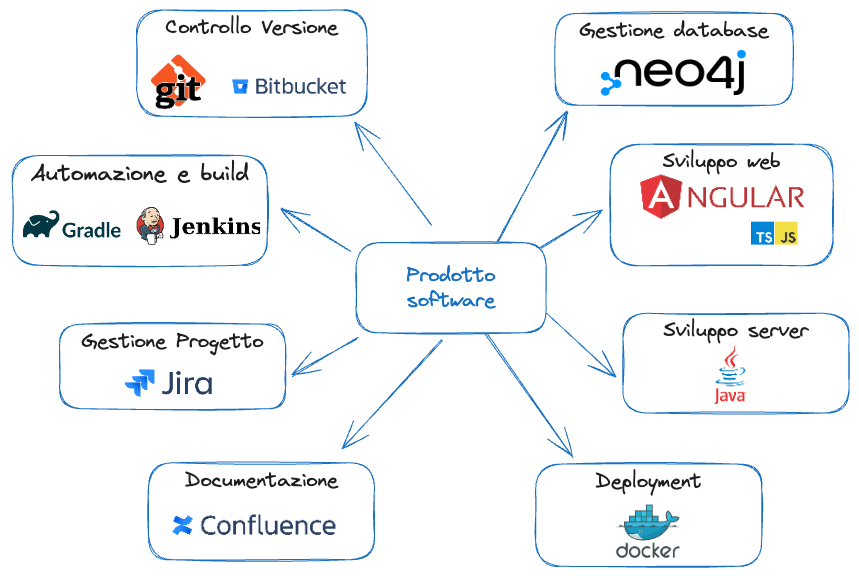
\includegraphics[width=1\columnwidth]{diagramma_strumenti} 
  \caption{Strumenti utilizzati}
  \label{fig:diagramma_strumenti}
\end{figure}

I linguaggi di programmazione utilizzati hanno incluso:

\begin{itemize}
\item \textbf{Java:} La mia principale lingua di programmazione, utilizzata per lo sviluppo di applicazioni robuste e ad alte prestazioni, sia \textit{web} che desktop;

\item \textbf{JavaScript:} Fondamentale per lo sviluppo \textit{frontend}  , ha permesso di creare interfacce utente interattive e dinamiche;

\item \textbf{TypeScript:} Utilizzato per aggiungere tipizzazione statica a JavaScript, migliorando la leggibilità e la manutenibilità del codice;

\item \textbf{Groovy:} Impiegato per script e automazioni, sfruttando la sua compatibilità con la \gls{JVM} e la sua sintassi espressiva;

\item \textbf{Cypher:} Il linguaggio di \textit{query} per Neo4j, essenziale per interrogare e manipolare i dati nei nostri \textit{database} a grafo.
\end{itemize}

Questi strumenti e linguaggi hanno formato il nucleo della mia cassetta degli attrezzi di sviluppo, permettendomi di affrontare una vasta gamma di sfide tecniche e di contribuire efficacemente 
ai progetti dell'azienda.

\subsection{Convenzioni}
Nel corso dello sviluppo dei progetti che impiegano il \textit{frameworkg} interno, vengono adottate una serie di convenzioni standardizzate. 
Le convenzioni, archiviate in \textit{Confluence} per un facile accesso da parte di tutti i dipendenti, 
sono state pensate per garantire coerenza, efficienza e qualità nel lavoro. Sono categorizzate come segue:

\begin{itemize}
\item \textbf{Documentazione:} Regole che stabiliscono come documentare efficacemente il codice sorgente. 
L'obiettivo è assicurare che ogni segmento di codice sia accompagnato da commenti chiari e concisi, che ne spieghino la funzione e la logica. 
Questo approccio, non solo facilita la comprensione del codice da parte di altri sviluppatori, ma è anche fondamentale per la manutenzione a lungo termine del \textit{software};

\item \textbf{Scrittura analisi:} Linee guida delineano il metodo per redigere analisi dei requisiti e progettazione delle strutture di basi di dati. 
L'obiettivo è garantire che le analisi siano scritte in modo chiaro e strutturato, facilitando la comprensione e la comunicazione tra i membri del \textit{team} e con i clienti;

\item \textbf{Progettazione:} Regole forniscono indicazioni su come progettare i componenti \textit{software}. 
L'enfasi è posta sulla creazione di \textit{design} modulari e riutilizzabili, che facilitano la manutenzione e l'estensione del codice nel tempo. 
Questo approccio aiuta a ridurre la complessità del codice e a migliorare la scalabilità delle applicazioni;

\item \textbf{Codifica:} Convenzioni che mirano a standardizzare lo stile di codifica. L'obiettivo è scrivere codice in modo uniforme, seguendo un insieme di regole che ne migliorino la leggibilità e la comprensione. Questo include convenzioni su nomi di variabili, strutture di controllo, formattazione del codice e commenti;

\item \textbf{Versionamento:} Regole stabiliscono come gestire il versionamento del codice sorgente. 
L'obiettivo è facilitare la tracciabilità delle modifiche e la gestione delle diverse versioni del \textit{software}. 
Questo è cruciale per il controllo qualità, la risoluzione dei \textit{bug} e la collaborazione tra i membri del \textit{team}.
\end{itemize}

Adottare convenzioni ha migliorato significativamente la qualità e l'efficienza del processo di sviluppo. Hanno fornito una base solida per la collaborazione e la standardizzazione, elementi chiave per il successo dei nostri progetti \textit{software}.
\section{Rapporto con l'innovazione}

\noindent{\azienda} si impegna costantemente nell'innovazione delle aziende clienti, giocando un ruolo cruciale nella loro trasformazione digitale. 
Specializzata nella progettazione e realizzazione di soluzioni integrate, l'azienda si dedica alla riorganizzazione dei processi aziendali e 
professionali, mirando a un impatto significativo e misurabile. \\
\noindent Per perseguire questo obiettivo, {\azienda} investe una quota sostanziale del proprio fatturato, tra il 15 e il 20\%, 
in Ricerca e Sviluppo ogni anno. L'investimento testimonia l'impegno dell'azienda nel rimanere all'avanguardia nel settore tecnologico, 
garantendo l'innovazione continua dei suoi prodotti e servizi. \\
\noindent Un aspetto distintivo di {\azienda} è la sua capacità di ascoltare e valorizzare le idee provenienti da clienti, dipendenti e collaboratori. 
Questo approccio collaborativo è fondamentale per l'ispirazione e lo sviluppo di nuovi prodotti e soluzioni innovative. Attualmente, quasi tutti i 
prodotti installati presso i clienti sono in fase di aggiornamento, dimostrando l'impegno dell'azienda nel fornire soluzioni sempre aggiornate e 
allineate con le ultime tendenze tecnologiche. \\
\noindent L'investimento in cultura e formazione è un altro pilastro fondamentale per {\azienda}. Ogni anno, l'azienda organizza una serie di corsi 
di formazione per i propri dipendenti, consentendo loro di acquisire competenze su nuove tecnologie e strumenti. 
I corsi sono tenuti sia da membri esperti del team interno, sia da consulenti esterni, e spesso si avvalgono di piattaforme 
di \textit{e-learning} come \textit{Udemy Business}, fornite gratuitamente dall'azienda. \\
\noindent In aggiunta, {\azienda} promuove attivamente l'innovazione attraverso l'organizzazione di eventi, 
come il \textit{Choose Innovation} in collaborazione con \textit{IBM}. Gli eventi rappresentano un'opportunità per discutere di 
innovazione e di come le aziende possano adottare nuove strategie per rimanere competitive nel mercato in rapida evoluzione. 
Attraverso questi sforzi, {\azienda}, non solo rafforza la propria posizione come \textit{leader} nell'innovazione, ma contribuisce anche 
attivamente all'avanzamento del settore. \\